\chapter{Introduction}
\label{ch:intro}

This thesis presents a mechanical engineering perspective on the investigation into the fabrication and alignment of a \acf{DVP} which is a component of the \acf{AFIT} \acf{CTEx}. The work herein investigates mechanical limitations in fabricating and aligning a \ac{DVP} assembly by utilizing optical diagnostic tools to drive systematic mechanical design. \ac{CTEx} is a long-running \ac{AFIT} research effort to promote space-based \acf{CTI} technology utilizing a rotating prism as the dispersive element in the optical system~\cite{Lemaster,Dearinger, Gustke, Gould}~\cite{ODell, ODellSPIE, Niederhauser}.

%This work was intended as an open-ended investigation and only the pertinent theory and observations as they pertain to the advancement of the CTEx project are detailed herein.

%%%%%%%%%%%%%%%%%%%%%%%%%%%%%%%%%%%%%%%%%%%%%%%%%%%%%%%%%%%%%%%%%%%%%%%%%%%%%%%%%%
\section{Motivation}
\label{sec:motivation}

 \ac{CTEx} is motivated by the spectroscopic capabilities of spinning-prism \ac{CTI} technology above the industry-leading imaging Fourier transform spectroscopy (imaging FTIR) approaches. The most significant advantages are presented in~\cite{Bostick08} by Bostick and Perram whose claim is that ``chromotomography offers several advantages over FTIR approaches, including: (1) simple design with less sensitivity to vibration, (2) easy integration with standard imaging sensors, and (3) the use of event phenomenology in the CT transform for increased temporal response"~\cite[p. 519]{Bostick08}. \ac{CTEx} achieves \ac{CTI} by utilizing a rotating \ac{DVP} dispersive element. An alternative approach to achieving \ac{CTI} is to use a non-rotating dispersive element and large optical detector arrays~\cite{Descour}. While each method of achieving \ac{CTI} offer advantages, the objective of \ac{CTEx} includes a spectral resolution of transient events that is not obtained by non-rotating designs. Further detail on the advantages of \ac{CTI} is presented in Section~\ref{sec:HSIres}.

Previous \ac{CTI} experiments conducted at \ac{AFIT} used prisms characterized by direct angle observations implemented to detail a wavelength-dependent dispersion profile. However, with the completion and operation of recent \ac{CTI} instruments by \ac{AFIT}, the limitations imposed on \ac{CTI} efficacy by the misalignment of the optical system were highlighted~\cite{Sue} \cite{Bostick}. The inability to reconstruct a fast-transient scene has been largely attributed to the fabrication and alignment imperfections in the \ac{DVP} and so inspire improvement of the techniques for realizing a spinning \ac{DVP} optical element \cite{HawksATF}. As is demonstrated by Bostick~\cite{Bostick}, the fabrication and installation alignment of the \ac{DVP} assembly has significant impact on the spatial and spectral information that can be obtained by the \ac{CTI} system. With new understanding as a result of \ac{AFIT} research efforts gone before, the need is established for a thorough investigation set on achieving an understanding of the practical limitations in precision installation alignment and fabrication of a \ac{DVP}.

%%%%%%%%%%%%%%%%%%%%%%%%%%%%%%%%%%%%%%%%%%%%%%%%%%%%%%%%%%%%%%%%%%%%%%%%%%%%%%%%%%
\section{Hyperspectral Remote Sensing}
\label{sec:hyperspectralRemoteSensing}

The \ac{CTEx} instrument is a proposed space-based hyperspectral remote sensor. An introduction to hyperspectral remote sensing is offered here beginning with a description of remote sensing in general.

\subsection{Remote Sensing}
\begin{quote}
Remote sensing is the science of deriving information about an object from measurements made at a distance from the object, i.e., without actually coming into contact with it. The quantity most frequently measured in present-day remote sensing systems is the electromagnetic energy emanating from the objects of interest... (D. A. Landgebe, quoted in Swain and Davis, 1978, p. 1) \cite{Campbell}
\end{quote}

The electromagnetic (EM) energy spectrum, in general, is the broad range of electromagnetic radiation defined by the frequency at which the energy oscillates perpendicular to the path it dominantly traverses. A spectral band, or spectrum, refers to a specified range of frequencies (or wavelengths) at which electromagnetic waves exist. As the total electromagnetic spectrum is continuous, the approximate extent of these ranges is often defined by common physical boundaries. For example, the visible spectrum is defined by the approximate range of electromagnetic radiation that is detectable by the human eye \cite{Hecht}. The ranges are illustrated in Figure~\ref{fig:EMspectrum} and detailed in Table~\ref{tbl:EMspectrumTable}, however, the range of each spectrum is specified differently by various references as each range is intractable due to a lack of universally-recognizable constraints. Throughout this work, where the wavelength of energy is used to classify a spectrum, the assumed medium is a vacuum because, overall, the frequency of electromagnetic energy remains constant, but the wavelength changes relative to the medium in which it travels according to Equation~\eqref{eq:wavelength}~\cite{Hecht}.

\begin{figure}[htb]		% EMspectrum
\centering
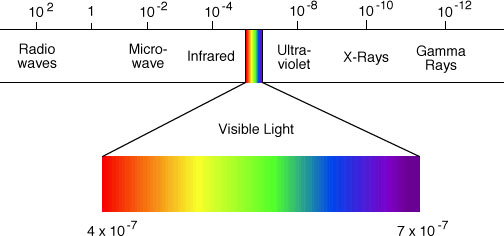
\includegraphics[width=0.75\textwidth]{images/chap1/EMspectrum}
\caption{Illustration of \acl{EM} spectrums with the visible spectrum highlighted~\cite{RedOrbit}.}
\label{fig:EMspectrum}
\end{figure}

\begin{table}[htb] 		% EMspectrumTable
\caption{Principle Divisions of the EM Spectrum} % title of Table 
\label{tbl:EMspectrumTable}
\centering % used for centering table 
\begin{tabular}{lr} % centered columns (2 columns)
\hline
Division & Limits \\  % inserts table heading 
\hline % inserts single horizontal line
Gamma Rays & less than 0.03 $nm$ \\
X-Rays & 0.03 - 300 $nm$\\
Ultraviolet Radiation & 0.30 - 0.38 \textmu m \\
Visible Light & 0.38 - 0.72 \textmu m \\
Infrared Radiation & 0.72 - 1000 \textmu m \\
 \hspace{.25cm} $\bullet$  Near infrared & 0.72 - 1.30 \textmu  m \\
 \hspace{.25cm} $\bullet$  Mid infrared & 1.30 - 3.00 \textmu  m \\
 \hspace{.25cm} $\bullet$  Far infrared & 7.00 - 1000 \textmu  m \\
Microwave Radiation & 1 - 300 $mm$ \\
Radio Waves & greater than 30 $cm$ \\
\end{tabular} 
\end{table}

\begin{table}		% eq:wavelength
\centering
\begin{equation}		% wavelength
\label{eq:wavelength}
\lambda = \frac{\nu}{f}
\end{equation}
\begin{tabular}{lll}
\singlespace
$\lambda$ & $\equiv$ & $\textit{wavelength in a medium}$ \\
$\nu$ & $\equiv$ & $\textit{speed of EM wave in a given medium}$ \\
$f$ & $\equiv$ & $\textit{frequency of the EM wave}$ \\
\end{tabular}
\end{table}

\subsection{Spectroscopy}
Spectroscopy is the study of electromagnetic waves separated by energy level, i.e. wavelength~\cite{Kulesa}. Spectroscopy enables the identification of chemical elements, in many cases, by direct, passive observation of electromagnetic waves as certain elements emit energy at sharply-defined wavelengths when chemical reactions occur or reflect only some wavelengths. Figure~\ref{fig:HgLampSpectrum} displays the amplitude of the energy released across the visible spectrum by current conducting through a mercury vapor lamp~\cite{Roberts}. The response profile is unique and, therefore, valuable, as there is no other event that emits energy with the exact same spectral profile. As such, this general event of current conducting through mercury vapor is positively identified by observation of its distinct emission. The unique wavelength profiles of emission or reflection for a material or event are known as spectral signatures~\cite{SpectralSignatures}.

\begin{figure}[htb]		% HgLampSpectrum
\centering
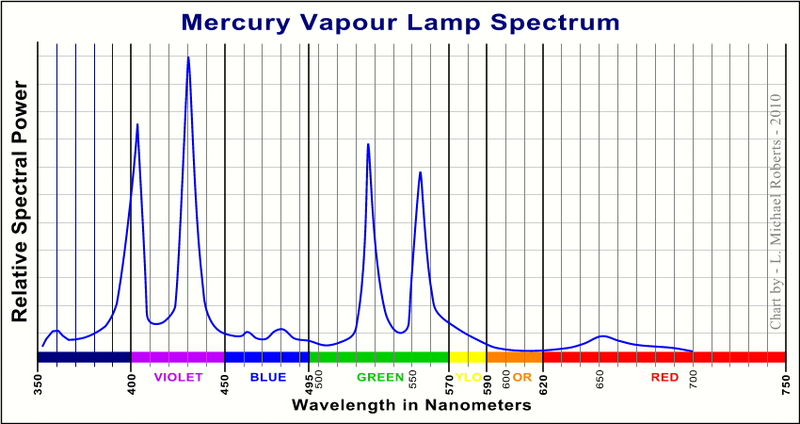
\includegraphics[width=.9\textwidth,trim=.1cm .1cm 2cm 1cm,clip]{images/chap1/HgLampSpectrum}
\caption{Spectral Signature of a mercury vapor lamp. The specific profile of power vs. wavelength shown is unique to the mercury vapor lamp~\cite{Roberts}.}
\label{fig:HgLampSpectrum}
\end{figure}

\subsection{Hyperspectral Remote Sensing}
\label{sec:HSI}
Hyperspectral remote sensing refers to the use of spectroscopy for observation of electromagnetic radiation within a uniquely-prescribed spectral band. To be considered hyperspectral, the energy observed must radiate at 0.4 to 14 \textmu m wavelength (20 to 750 THz frequency)~\cite{Sue} which encompasses the entire visible spectrum as well as parts of the \ac{SWIR} and the ultraviolet spectrums. The propensity for earth-imaging spectrometers to observe in the hyperspectral bandwidth is attributed to the assiduous tendency of the Sun to illuminate the Earth. The significance of solar illumination is evident in Figure~\ref{fig:RemoteSensing} showing that the energy detected by an Earth-observing satellite is largely the Sun's reflected radiation. Figure~\ref{fig:SolarEmissionSpectrum} shows that the greatest magnitude of received solar radiation occurs inside the hyperspectral bandwidth. Because the earth is illuminated by the hyperspectral bandwidth, it also reflects significantly in the hyperspectral bandwidth supplying ample signal for remote-sensing instruments. Furthermore, hyperspectral imagers are distinguished from other imagers by boasting a significantly higher spectral resolution than do other earth-sensing spectrometers~\cite{Shippert}. Greater spectral resolution is defined by more numerous and more narrow bandwidths within the designated spectrum. Higher spectral resolution allows for more precise definition of the signal received. Figure~\ref{fig:Reflectance} illustrates the spectral information inherent to an observed scene.

% note: "radiation" is the process of waves travelling, "emission" is the process of generating those radiation waves

\begin{figure}[htb]		% RemoteSensing
\centering
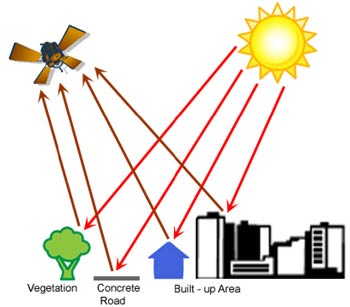
\includegraphics[width=0.5\textwidth]{images/chap1/RemoteSensing}
\caption{The radiation detected by an Earth-observing satellite has a significant contribution from solar emission~\cite{RemoteSensing}.}.
\label{fig:RemoteSensing}
\end{figure}

\begin{figure}[htb]		% SolarEmissionSpectrum
\centering
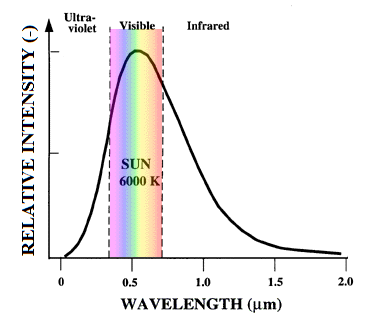
\includegraphics[width=0.5\textwidth]{images/chap1/solaremissionspectrum}
\caption{The solar emission spectrum indicates that most of the solar radiation reaching earth is in the low-end of the hyperspectral region of 0.4 to 14 \textmu m~\cite{JunkScience}.}
\label{fig:SolarEmissionSpectrum}
\end{figure}

% From a sampling-theory perspective, assuming equally-spaced, adjacent bandwidths, the spectral resolution or, the bandwidth of each spectral slice, defines the Nyquist frequency for the sampled signal. If the detected signal intensity vs. frequency curve contains frequency contribution above the Nyquist frequency, then the signal representation is degraded due to aliasing. With this relationship, the required bandwidth is be chosen based on an estimated signal profile of the desired targets. This is especially important as the transmittance of the atmosphere varies with the wavelength. This concept is illustrated in figure~\ref{fig:Reflectance}.

\begin{figure}[htb]		% Reflectance
\centering
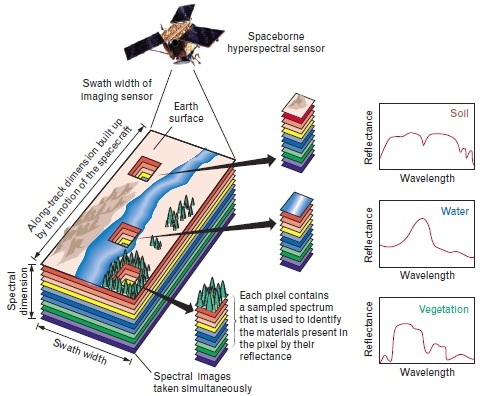
\includegraphics[width=1\textwidth]{images/chap1/ReflectanceSpectrum}
\caption{Spectral signature inherent to the scene at various points sensed by a hyperspectral imager~\cite{Shaw}.}
\label{fig:Reflectance}
\end{figure}

\subsection{The Hypercube}
A hyperspectral imager extracts from a signal the intensity of numerous finite spectral bandwidths at discrete points within the field of view. To visualize these datasets, the hypercube is often presented as shown in Figure~\ref{fig:hypercube}, which is ground image data collected by the \ac{AVIRIS}. Each horizontal slice through the XY-plane of the hypercube displays the intensity of a particular bandwidth as it varies with location in the two-dimensional \ac{FOV}. The ideal hypercube presents a two-dimensional spatial distribution of signal intensity at each infinitesimal wavelength along the Z-direction, or a continuous variation in the spectrum.

\begin{figure}[htb]		% hypercube
\centering
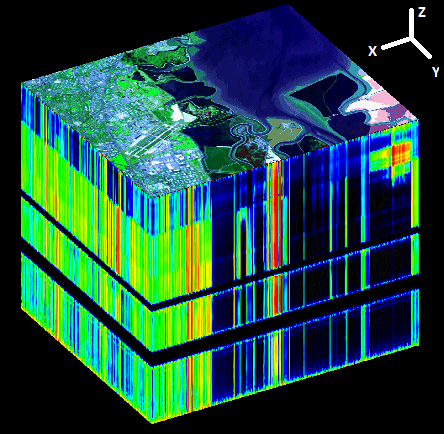
\includegraphics[width=0.75\textwidth]{images/chap1/avcubebig}
\caption{Hypercube taken from AVIRIS platform over Moffet Field, CA. Each cross section parallel to the XY-plane is the two-dimensional spatially-resolved emission intensity over the field of view at an infinitesimal spectral band. The wavelength of the energy varies continuously in the Z-direction~\cite{AVIRIS}}.
\label{fig:hypercube}
\end{figure}

\subsection{Hyperspectral Imager Temporal Resolution}
\label{sec:HSIres}
The performance measure of temporal resolution is not often discussed in relation to spectroscopy. However, it is an important aspect of hyperspectral imaging as many interesting targets evolve quickly both spectrally and spatially. To illustrate the relationship between spatial, spectral, and temporal resolution, examples are mapped onto a resolution triangle in Figure~\ref{fig:trifecta}. A hypercube is shown on the left and represents a spectrally- and spatially-resolved, two-dimensional static scene with low temporal resolution as the whole image is not associated with any one instant in time. An explosion is shown on the right and represents a spatially- and temporally-resolved event with no spectral-resolution beyond the color bands of the detector array. A chart of spectral change over time at the bottom is resolved for a finite area and offers no spatial resolution over the area. Because most imagers naturally exclude one element of the resolution triangle, some information is inherently lost. For hyperspectral imagers, the temporal aspect is most often traded for the information in the spatially- and spectrally-resolved hypercube. A closer look at hyperspectral imager instrumentation operation reveals the natural temporal exclusion.

\begin{figure}[htb]		% trifecta
\centering
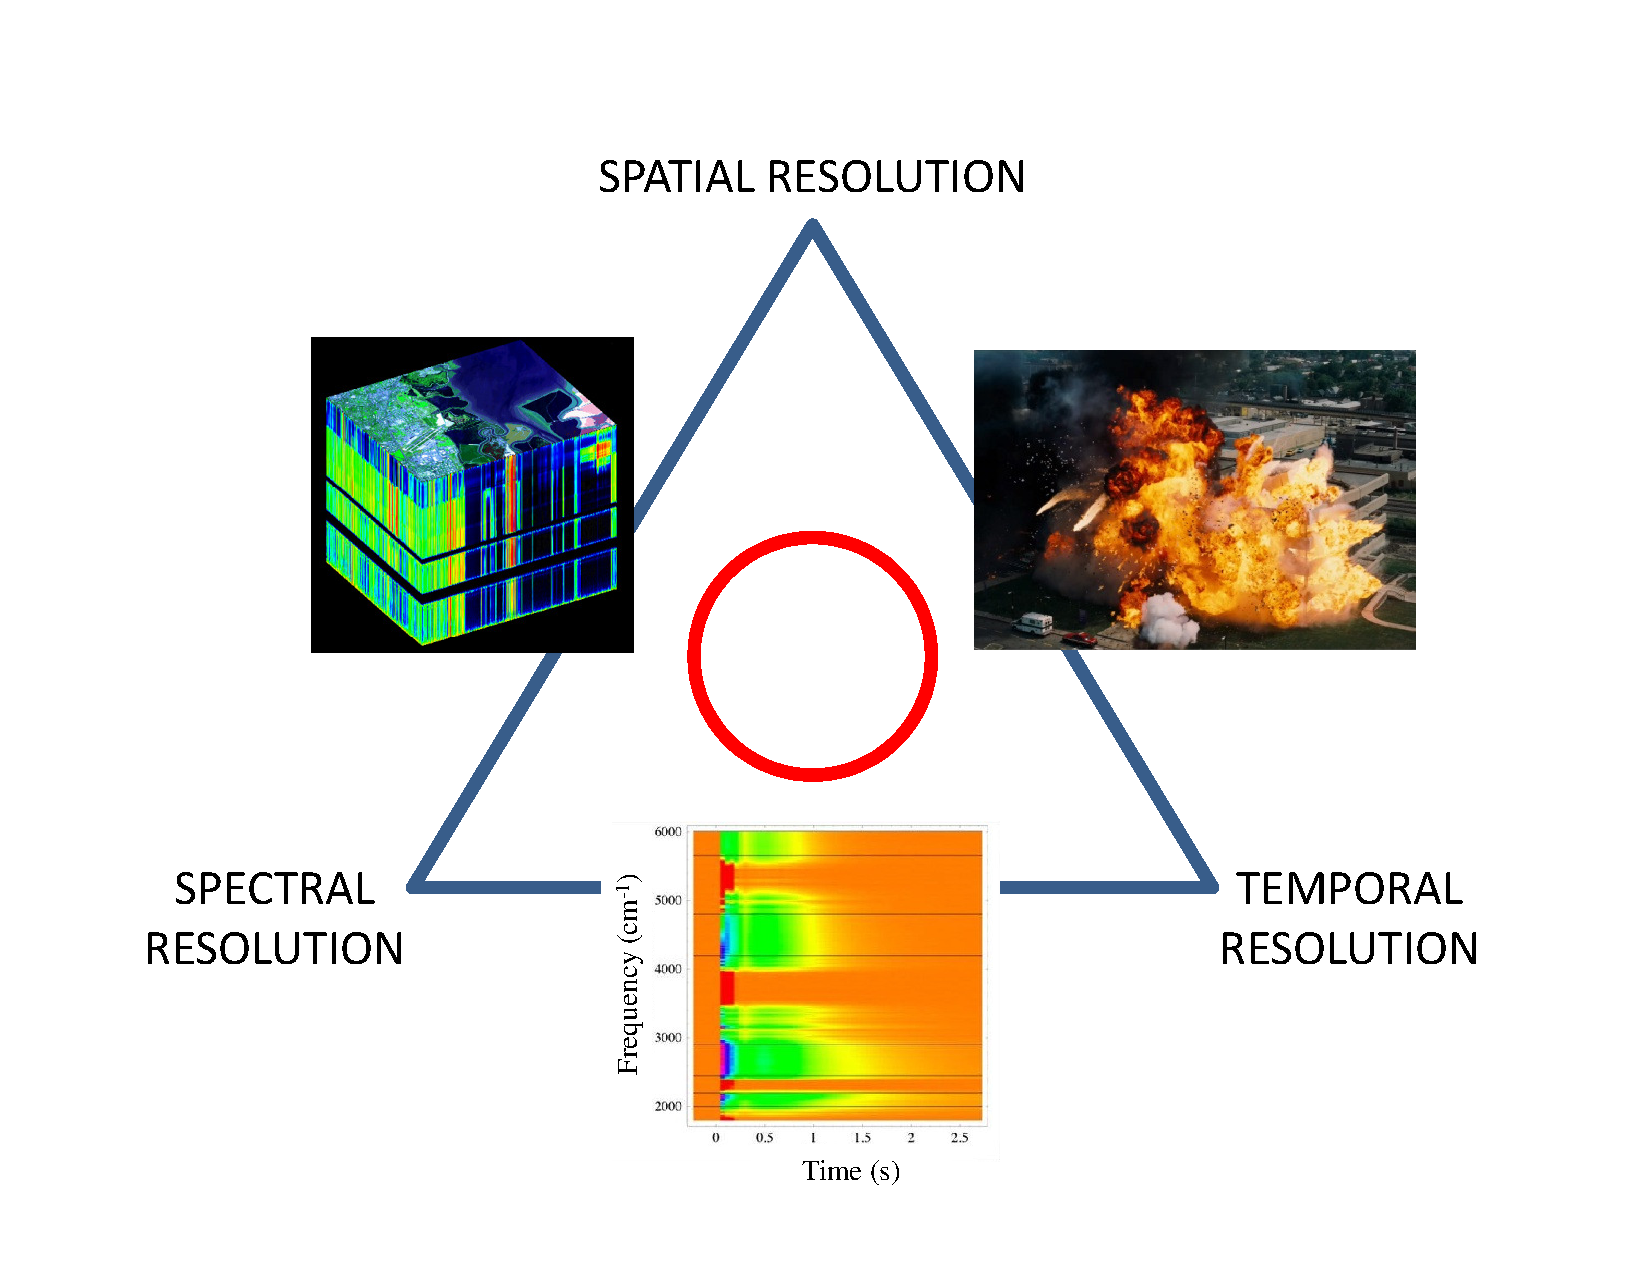
\includegraphics[width=1\textwidth,page=1]{images/chap1/MyGraphics_Ch1}
\caption{The resolution triangle illustrates the natural trades in image system resolution. Although not limited by general theory, realized imaging systems tend to achieve high resolution in only one or two of the three resolution types. CTI technology transcends this limitation~\cite{Niederhauser,DarkKnight}}.
\label{fig:trifecta}
\end{figure}

As discussed in Section~\ref{sec:hyperspectralImagers}, there have been and currently exist a number of space-based, earth-observing hyperspectral imagers. These imagers, by definition, generate highly-resolved intensity distributions as a function of spatial and spectral dimensions visualized by the hypercube of Figure~\ref{fig:hypercube}. The limitation of these and most spectrometers is that the time to collect the data to generate a spatially- and spectrally-resolved hypercube for a large \ac{FOV} is long enough that rapidly-changing events are not resolved temporally. Consider an imager such as EO-1 Satellite's Hyperion Imaging Spectrometer. This instrument operates as a push-broom spectrometer able to spectrally resolve a one-dimensional landscape as shown in Figure~\ref{fig:pushbroomOperation}. Because Hyperion and other push-broom spectrometers must resolve only individual thin slices of the \ac{FOV} at one time, the hypercube for the entire \ac{FOV} takes considerable time to integrate. If an explosion occurred within some segment of a two-dimensional area, Hyperion would either miss the event or only collect incongruous spectral information along one spatial line. 

 The solution to this temporal lapse is \ac{CTI}. The rapidly-rotating dispersion element projects the spectral information onto a spatial dimension and records, in multiple images, resolved spectral and spatial information for the hypercube many times per second. With implementation of \ac{CTI}, a space-based observer has the ability to survey a large ground swath area continuously and resolve spatial and spectral changes with time at any point within the \ac{FOV}. Thus, \ac{CTI} reaches all three corners of the resolution triangle in Figure~\ref{fig:trifecta}.
 
 \begin{figure}[htb]		% pushbroomOperation
\centering
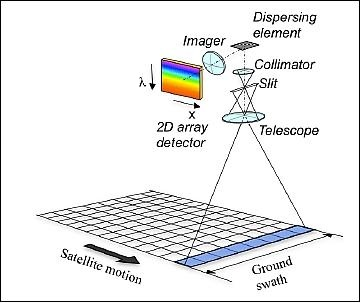
\includegraphics[width=0.5\textwidth,trim=0.25cm 0.25cm 0.25cm 0.25cm,clip]{images/chap1/pushbroomOperation}
\caption{A push-broom spectrometer resolves one narrow strip within the field of view at each integration~\cite{AVIRIS}}.
\label{fig:pushbroomOperation}
\end{figure}

\subsection{CTI Disadvantages}
Though \ac{CTI} offers resolution capabilities not achieved by other technologies, the advantages are not easily attained. As evidenced by the hard-earned advancement of the technology, \ac{CTI} hardware and theory is wrought with many intricacies and is highly-sensitive to numerous subtleties in instrument design and image processing. Pertinent to the research presented herein, it is shown that small imperfections and uncertainties in \ac{DVP} fabrication result in highly degraded results. \ac{CTI} relies on the alignment of optical components to sub-wavelength precision. While this is obviously accomplished in countless optical systems, few must maintain these tolerances while combating the disturbances of the \ac{DVP} rotating at high speed.

%%%%%%%%%%%%%%%%%%%%%%%%%%%%%%%%%%%%%%%%%%%%%%%%%%%%%%%%%%%%%%%%%%%%%%%%%%%%%%%%%%
\section{Research Goals}

The main goal for the research presented is an investigation into the \ac{DVP} optical element to further the \ac{CTEx} research effort at \ac{AFIT}. With several successful displays of rotating-prism \ac{CTI}, the technology is ready to support a laboratory-based working system which integrates components having the exact optical properties of the proposed space-based \ac{CTEx}. The nominal optical design of a four-piece \ac{DVP} has been completed, but it remains to be determined how well a fabricated \ac{DVP} is able to match the mechanical design and how well the as-built configuration is able to be characterized. The first step in qualifying the fabrication is to develop measurement techniques which define the geometry of the prism assembly to sub-wavelength precision. The specific goals are listed below.

% \begin{itemize}
% \singlespace
% \item{Develop optical diagnostic processes for \ac{DVP} measurement and model verification}
% \item{Develop a method to define the geometry of a prism assembly at sub-wavelength precision using interferometer measurements}
% \item{Develop a method of determining \ac{DVP} fabrication tolerance specifications}
% \item{Present the \ac{AFIT} \ac{CTEx} \ac{DVP} design methodology}
% \item{Design a DVP interface for the existing \ac{DVP} design and motor hardware}
% \end{itemize}

\begin{itemize}
\singlespace
\item{Investigate measurement techniques for a \acl{DVP} assembly}
\item{Establish a diagnostic method to characterize a \acl{DVP} assembly}
\item{Develop a method for specifying \acl{DVP} fabrication tolerances}
\item{Propose a prism sleeve design for the \acl{DVP} and motor interface}
\end{itemize}


%%%%%%%%%%%%%%%%%%%%%%%%%%%%%%%%%%%%%%%%%%%%%%%%%%%%%%%%%%%%%%%%%%%%%%%%%%%%%%%%%%
\section{Organization}

Chapter~\ref{ch:bkgnd} reviews the history of \ac{CTI} and the experiments conducted by industry as well as at \ac{AFIT}. Chapter~\ref{ch:bkgnd} also details the history that has developed the need for this investigation into \ac{DVP} fabrication and characterization. Chapter~\ref{ch:applicableTheory} reviews the physics and methodology pertinent to the development and results of the experiments performed. Chapter~\ref{ch:DVP}  applies the theory to the performed experiments and reveals the results of the experiments for \ac{DVP} characterization. Chapter~\ref{ch:DVP} also presents a design for the \ac{CTEx} \ac{DVP} holder and the methodology of its design. Chapter~\ref{ch:conclusion} draws conclusions from the results and observation of experiments and proposes future work able to utilize and build upon the conclusions drawn from research herein.
